please note the naming pattern of source files:

excercise X task Y part Z = eXtYpZ

\section{Task 1}
see \verb|ex1.cpp|

\subsection{square test}
square plot, see fig \ref{fig:square}
\begin{figure}[b]
  \centering
  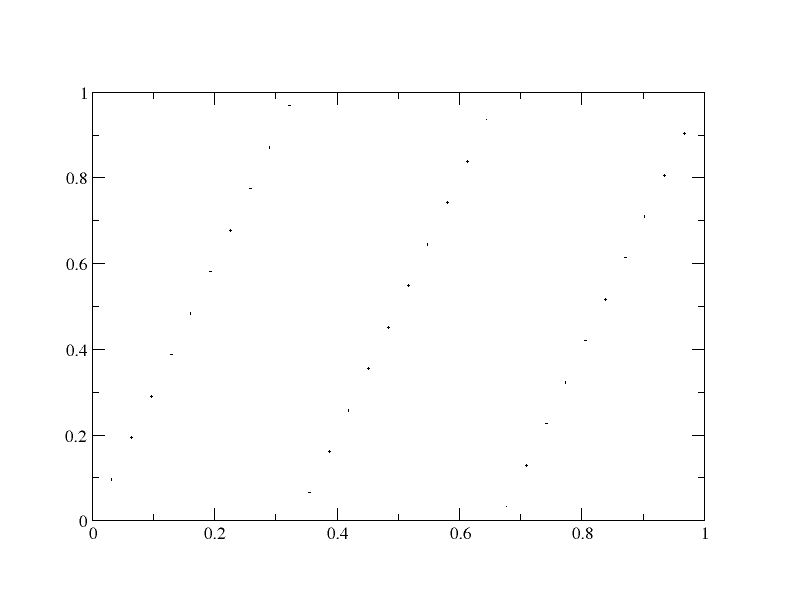
\includegraphics[width=\textwidth]{square1.png}
  \caption{squareplot}
  \label{fig:square}
\end{figure}

max number of points:


\subsection{3d plot}
cubeplot, see fig \ref{fig:cube} and \verb|ex12.cpp|

with n = 100000; c = 3; p = 31; $x_{seed}$ = 1

created with matlab \verb|plot3(rnd3d(:,1),rnd3d(:,2),rnd3d(:,3),'.')|

\begin{figure}
  \centering
  \includegraphics[width=\textwidth]{cube1.png}
  \caption{cubeplot}
  \label{fig:cube}
\end{figure}


\subsection{other random number generator}
see \verb|ex12.cpp|, fig \ref{fig:square2} and fig \ref{fig:cube2}

\begin{figure}[b]
  \centering
  \includegraphics[width=\textwidth]{square2.png}
  \caption{squareplot with }
  \label{fig:square2}
\end{figure}

\begin{figure}[b]
  \centering
  \includegraphics[width=\textwidth]{cube2.png}
  \caption{cubeplot with }
  \label{fig:cube2}
\end{figure}


\section{Task 2}
skech of idea, using cartesian coordinate system:
\begin{itemize}
  \item generate a pair of homogeneous random points $(x_1,x_2)$, with $x_i \in [-1,1]$
  \item if $x_1^2 + x_2^2<=1$, then return the point, otherwise reject it and try again
  \item if necessairy, transform to polar coordinate system
\end{itemize}
see \verb|ex1task2.cpp| and plot \ref{fig:ex1task2}.

\begin{figure}[b]
  \centering
  \includegraphics[width=\textwidth]{ex1task2.png}
  \caption{cubeplot with }
  \label{fig:ex1task2}
\end{figure}


\section{Task 3}
see \verb|ex12.cpp|, used $k=10$ bins, $n=1000$ binned random numbers.
\begin{itemize}
  \item $c = 3$; $p = 31$; $x_\mathrm{seed} = 1$: $\chi^2 = 0.1$
  \item $c = 1017$; $p = 8191$; $x_\mathrm{seed} = 154$: $\chi^2 = 5.54$
  \item built in \verb|rand()| (using init. \verb|srand(670706)|) $\chi^2 = 13.74$
\end{itemize}
